% IEEE JSTARS manuscript. Build: tectonic -X compile main.tex  (or pdflatex + bibtex)
% Every number traces to a report file; REPRODUCE.md maps sections to the scripts that write them.
\documentclass[journal]{IEEEtran}
\usepackage{iftex}
\ifPDFTeX\usepackage[utf8]{inputenc}\fi
\usepackage[T1]{fontenc}
\usepackage{amsmath,amssymb}
\usepackage{textcomp}
\usepackage{newunicodechar}  % lets the source use these symbols under both pdfLaTeX and XeTeX
\newunicodechar{−}{\ensuremath{-}}
\newunicodechar{Δ}{\ensuremath{\Delta}}
\newunicodechar{ρ}{\ensuremath{\rho}}
\newunicodechar{→}{\ensuremath{\rightarrow}}
\newunicodechar{±}{\ensuremath{\pm}}
\newunicodechar{≥}{\ensuremath{\geq}}
\newunicodechar{≤}{\ensuremath{\leq}}
\newunicodechar{×}{\ensuremath{\times}}
\newunicodechar{–}{--}
\newunicodechar{—}{---}
\newunicodechar{²}{\ensuremath{^2}}
\newunicodechar{σ}{\ensuremath{\sigma}}
\usepackage{graphicx}
\usepackage{booktabs}
\usepackage{multirow}
\usepackage{array}
\usepackage[hidelinks]{hyperref}
\usepackage{cite}
\usepackage{xcolor}
\graphicspath{{../../figures/}}

\newcommand{\iouf}{IoU$_\text{flood}$}
\newcommand{\ci}[2]{[#1,\,#2]}
\newcommand{\todo}[1]{\textcolor{red}{[#1]}}

\begin{document}
\bstctlcite{IEEEexample:BSTcontrol}

\title{Terrain Helps SAR Flood Mapping on New Floods, and Same-Event Splits Hide It}

\author{Jeremy~Ky, Bao~Duong, and~Rich~Nguyen%
\thanks{The authors are with the University of Virginia, Charlottesville, VA 22904 USA (e-mail:
juh7hc@virginia.edu; rjr6zk@virginia.edu; nn4pj@virginia.edu). Corresponding author: Jeremy Ky.}%
\thanks{Code: \url{https://github.com/jeremyky/SAR-Flood-Terrain}.}}

\markboth{Preprint}%
{Ky \MakeLowercase{\textit{et al.}}: Terrain helps SAR flood mapping on new floods}

\maketitle

\begin{abstract}
Flood segmentation models for Sentinel-1 radar must work on new floods, yet they are usually tested on
images from the flood events they were trained on. We show that this hides the value of terrain. A U-Net
trained on the 11 events of Sen1Floods11 gains almost nothing from height above nearest drainage on that
dataset's own test split (+0.007 intersection over union) but +0.128 on its held-out Bolivia event. On 79
external Copernicus emergency activations, the same input raises mean event intersection over union from
0.574 to 0.635 for water and from 0.317 to 0.349 for flooded area, with water improved on 69 of the 79 events, and the
gain holds without a threshold and under the benchmark's pre- and post-event protocol. It needs the right
terrain for the place: elevation and slope recover only a quarter of it, its event-level gain vanishes when
the drainage input is shifted by 500 m, blurred, or taken from another flood, and a model trained on such mismatched
input gains nothing. A fine-tuned 101-million-parameter foundation model benefits about as much and,
without the input, does not match the 7.8-million-parameter U-Net that has it. Used as a physics-based loss
or a mask, the same terrain does nothing. Trained on 159 events, the flood-extent gain is no longer
detectable, although a pre-registered test did not confirm a steady decline with the number of events. With
few labelled floods, terrain is a cheap gain that same-event evaluations miss.
\end{abstract}

\begin{IEEEkeywords}
Flood mapping, synthetic aperture radar, terrain, domain generalization.
\end{IEEEkeywords}

\section{Introduction}
\IEEEPARstart{S}{ynthetic} aperture radar (SAR) maps floods through cloud and at night, which makes
Sentinel-1 the workhorse of rapid flood mapping. Deep segmentation networks trained on labelled SAR
scenes now reach high accuracy on standard benchmarks, but a rapid-mapping model is always applied to a
flood it has not seen: a new river, a new landscape, a new season. Errors concentrate where backscatter
is ambiguous---radar shadow and layover in hilly terrain, smooth dry surfaces such as sand and tarmac,
wet soil, and vegetation over water---and which of these a model has learned to handle depends on the
floods it was trained on.

Terrain is the obvious physical prior. Water collects low and close to drainage, and elevation data are
global, free and available before the flood: the Copernicus GLO-30 digital elevation model
(DEM)~\cite{glo30dem} and the height above nearest drainage (HAND) derived from it~\cite{renno2008hand,
nobre2011hand,asfhand}. Physics-informed and physics-guided deep learning offers several ways to inject
such a prior: as an extra input, as a loss that penalizes physically implausible outputs, or as a
post-processing mask. Whether any of them helps on a \emph{new} flood is less clear than it may seem.
Most published comparisons use random or official tile splits of a single dataset, so training and test
tiles share flood events, and the comparison measures how well a model fits a known event rather than
how well it transfers.

This paper evaluates terrain priors where they matter, on flood events the model has not seen. We treat
the flood event as the unit of analysis throughout: we hold out whole events, score every event
separately, and compare model variants with paired statistics over events and over training seeds or
draws. Training on Sen1Floods11~\cite{bonafilia2020sen1floods11} and testing on 79 Copernicus Emergency
Management Service (CEMS) activations from GEOID-Flood~\cite{geoidflood} gives a test set large enough to
detect gains of a few points in intersection over union (IoU); training on subsets of GEOID-Flood's 159
training events shows how the value of terrain changes as more floods are labelled.

\begin{figure*}[t]
\centering
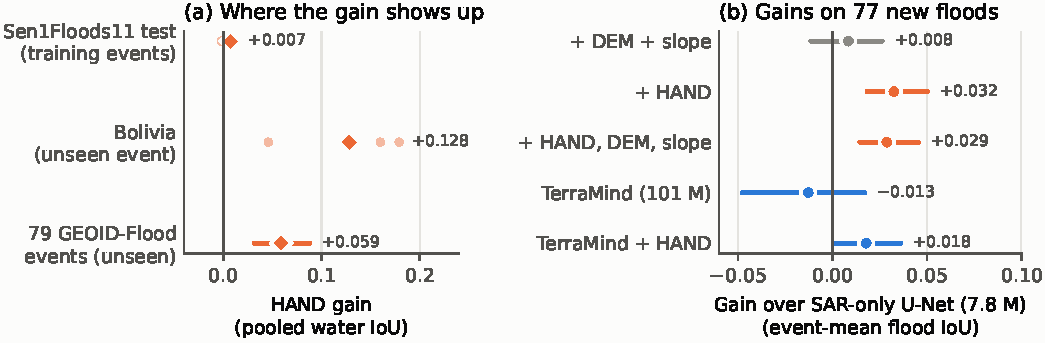
\includegraphics[width=\textwidth]{fig_overview.pdf}
\caption{Models trained on the 11 Sen1Floods11 events. (a) HAND gain in pooled water IoU on Sen1Floods11's
test split (tiles from the training events), its Bolivia hold-out and 79 external GEOID-Flood events (dots:
seeds; diamonds: means; bar: 95\% CI). (b) Gain over the SAR-only U-Net in event-mean flood IoU on 77
GEOID-Flood events (two-way 95\% CIs).}
\label{fig:overview}
\end{figure*}

Three findings stand out (Fig.~\ref{fig:overview}):
\begin{enumerate}
\item \emph{Same-event splits hide the value of terrain.} A U-Net trained on Sen1Floods11 gains almost
nothing from HAND on that dataset's official test split (+0.007 IoU), whose tiles come from the training
events, but +0.128 on its held-out Bolivia event and +0.059 in pooled water IoU over 79 external floods
(+0.061 in mean event IoU, improving 69 of them).
\item \emph{The gain needs correctly located, detailed height above drainage.} In this transfer, elevation
and slope recover only a quarter of it at the event level; shifting HAND by 500\,m in each axis,
blurring it, or swapping in another flood's HAND removes the event-level gain, and a model trained with mismatched HAND gains nothing, so it
is not a side effect of an extra input channel. A permanent-water map recovers none of the flood-extent
gain and, with many training events, teaches the model to look for water only where it already was.
\item \emph{A foundation model does not replace terrain.} HAND helps a fine-tuned 101\,M-parameter
TerraMind~\cite{jakubik2025terramind} about as much as it helps a 7.8\,M-parameter U-Net in event-mean
flood IoU (less for all water), and the small U-Net with HAND beats TerraMind without it.
\end{enumerate}

We also show that HAND as a physics loss or mask does nothing, even when the loss demonstrably enforces its
constraint; that the input gain survives threshold-free scoring, GEOID-Flood's own protocol and resampling
by country, and where it occurs by HAND, slope and land cover; that with 159 GEOID-Flood training events the
flood-extent gain is no longer detectable (a pre-registered test of a steady decline was null), while 500
tiles from all 159 events match all 8,712; and that two pre-registered remedies for HAND's failure cases do
not help. The full pipeline, run outputs and checkpoints are released.

\section{Related Work}

\subsection{Benchmarks and evaluation splits}
Sen1Floods11~\cite{bonafilia2020sen1floods11} provides 446 hand-labelled Sentinel-1 chips from 11 flood
events; its Bolivia event is the customary out-of-distribution test, but most work reports the official
split, in which test tiles come from the same events as training tiles. GEOID-Flood~\cite{geoidflood}
assembles CEMS rapid-mapping activations from 2016 to 2026 with a train/validation/test split by area of
interest (AoI) and a temporally disjoint held-out set of 2026 events. It benchmarks ImageNet and
geospatial foundation-model encoders (TerraMind, DOFA, OlmoEarth, SSL4EO and Satlas, each frozen and
fine-tuned) with a U-Net decoder; single-image Sentinel-1 models mostly reach an \iouf{} of 0.41--0.48 (one frozen encoder scores 0.21). It does
not vary the number of training events or test HAND.

\subsection{Terrain as an input}
Yadav \emph{et al.}~\cite{yadav2022attentive} fuse a 30-m SRTM DEM and a permanent-water layer with
Sentinel-1 on Sen1Floods11. Adding the DEM as a third channel slightly lowers IoU for their attentive
U-Net (0.672 to 0.661), while a two-stream fusion of DEM and permanent water gives their best result
(0.695); evaluation uses the Sen1Floods11 splits, not held-out events, and HAND is not used. GEOID-Flood
tests a DEM with a frozen TerraMind backbone on pre-event water-body delineation only and finds its effect
within noise. MSFlood-Net~\cite{msfloodnet} feeds SAR, optical, DEM and HAND to a ConvNeXt U-Net as
physically informed inputs on Gaofen data. ALTIS~\cite{altis} is a training-free change-detection
pipeline that uses HAND as a hard gate in a Bayesian fusion; on a single event (Hurricane Harvey),
removing HAND costs 0.052 IoU.

\subsection{Terrain on held-out events}
Two recent projects hold out Sen1Floods11 events. An unreviewed project~\cite{pranav2026loeo} runs
leave-one-event-out (LOEO) evaluation over all 11 events with a ResNet-34 U-Net and finds no reliable
terrain gain (macro IoU 0.564 for SAR versus 0.570 with HAND and slope; confidence intervals include
zero), as we do in Section~\ref{sec:loeo}; it does not test external events or vary the number of
training events. Chandrasiri and Liyanage~\cite{chandrasiri2026} hold out three events in turn with
VV/VH-only U-Nets and topology-aware metrics, without terrain.

\subsection{Physics-guided losses and cross-event generalization}
Gebre \emph{et al.}~\cite{gebre2026physics} combine a U-Net and a Fourier neural operator with
shallow-water residual losses and DEM-derived features, evaluated against hydrodynamic simulations. Our
losses are simpler output constraints on HAND, not partial-differential-equation residuals.
Kolluru \emph{et al.}~\cite{kolluru2026landcover} run Prithvi-EO-2.0~\cite{szwarcman2024prithvi} on 19
out-of-distribution events and find detection limited jointly by land cover and flood type, with part of
the error due to disagreement between reference products; they do not test terrain inputs.

\subsection{Gap}
We found no study that (a) tests a terrain prior on many external flood events, where 11-event LOEO is
underpowered; (b) compares terrain mechanisms---input, loss, mask---on held-out events with paired
event-level statistics; or (c) measures how the value of a terrain prior depends on the number of
training events, separately from the number of tiles.

\section{Data}
\label{sec:data}

\begin{table}[t]
\caption{Datasets}
\label{tab:data}
\centering
\footnotesize
\begin{tabular}{@{}p{0.17\columnwidth}p{0.33\columnwidth}p{0.40\columnwidth}@{}}
\toprule
 & Sen1Floods11 (hand-labelled) & GEOID-Flood \\
\midrule
Events & 11 & 159 train / 35 val / 82 test (80 used) / 9 held-out (2026) \\
Tiles & 446 chips, $512^2$ at 10 m & $1024^2$ UTM tiles at 10 m; 8,712 train, 2,635 test \\
SAR & S1 GRD VV/VH (dB) & post-event S1 GRD (linear $\sigma^0$ to dB); pre-event image per tile \\
Labels & water / not water & background / permanent water / flooded water \\
\bottomrule
\end{tabular}
\end{table}

Table~\ref{tab:data} summarizes the two datasets. For every tile we resample the Copernicus GLO-30
DEM~\cite{glo30dem} and the ASF GLO-30 HAND product~\cite{asfhand} bilinearly onto the tile's 10-m grid
and derive slope from the DEM; ESA WorldCover 2021~\cite{zanaga2022worldcover} is used only to describe
events.

\subsection{Label modes}
GEOID-Flood separates permanent from flooded water. We score it in two label modes: \emph{all water}
(permanent plus flooded, the Sen1Floods11 convention, which the Sen1Floods11-trained models were trained
to predict) and \emph{flooded water only} (permanent water ignored in scoring). We also
score GEOID-Flood's own protocol, which differences a pre- and a post-event prediction
(Section~\ref{sec:methods}).

\subsection{Overlap and cleaning}
CEMS activation EMSR388 is the Sen1Floods11 Spain 2019 flood and is excluded from the GEOID-Flood test
set. EMSR853's test AoI ships only a pre-event image, so 80 test events remain; 79 contain water and 77
contain flood. Of the 9,192 training tiles in the catalog, 254 are flagged invalid or are more than 95\%
nodata (which removes two events entirely, leaving 159 of 161), and 226 of the remaining 8,938 have no
post-event image or no label in the release, leaving 8,712. Sen1Floods11's Sri Lanka (EMSR205) and
Nigeria (EMSR314) events are in GEOID-Flood train; when GEOID-trained models are tested on Sen1Floods11,
we drop those events and Spain.

\subsection{Unseen activations}
GEOID-Flood splits by AoI, not by activation: 41 of the 80 test activations also have AoIs in the
training split, and 15 in validation. For GEOID-trained models we therefore report results on the 38
flood (39 all-water) test events whose activation does not appear in GEOID-Flood train (``unseen
activations''); results on all test events are given for completeness where they differ. The
Sen1Floods11-trained models share no event with GEOID-Flood test once EMSR388 is removed, so all 77/79
events are unseen for them.

\section{Methods}
\label{sec:methods}

\subsection{Models and inputs}
The main model is a U-Net~\cite{ronneberger2015unet} with four levels, base width 32 and channel
dropout 0.1 (7.8\,M parameters), trained from scratch. A ResNet-34 U-Net~\cite{he2016resnet} with
ImageNet weights (segmentation-models-pytorch~\cite{iakubovskii2019smp}) is the second backbone.
Section~\ref{sec:cd} adds a change-detection U-Net and Section~\ref{sec:fm} a TerraMind foundation
model. Inputs are scaled with fixed, data-independent transforms so that every event is treated
identically: VV and VH backscatter are clipped to $[-30, 5]$\,dB, shifted by $+12.5$\,dB and divided by 7.5\,dB;
HAND $h$ (metres) enters as $\log(1+h)/2$; the DEM enters as relief relative to the tile median, divided
by 50\,m and clipped to $\pm 3$; slope is divided by 15\textdegree. Pixels with any missing input are
ignored in training and scoring.

\subsection{Physics losses and post-processing}
All models minimize binary cross-entropy plus Dice loss. Two optional terms encode HAND as a physical
constraint on the output. The \emph{monotonicity} loss penalizes a pixel for being predicted wetter than
a pixel that lies lower above drainage: for pixel pairs $(a,b)$ a fixed stride apart along rows and
columns with $h_a - h_b \ge 1$\,m, it adds $\max(0, p_a - p_b - m)$ for predicted probabilities $p$ and
margin $m$, averaged over qualifying pairs. The \emph{ceiling} loss penalizes flood predicted above
15\,m HAND. As a post-processing baseline, every run is also scored with predictions above 15\,m HAND
set to dry.

\subsection{Training}
We use AdamW~\cite{loshchilov2019adamw} (learning rate $10^{-3}$, weight decay $10^{-4}$) with a one-cycle
schedule~\cite{smith2019superconvergence}, bf16 mixed precision, random flips and $90^\circ$ rotations,
and select the checkpoint with the best validation IoU. Sen1Floods11 models train for 100 epochs on
$256^2$ crops (batch 16) and validate on the official validation split or, for leave-one-event-out and
all-event training, on 15\% of the training chips. GEOID-Flood models
train on $512^2$ crops of the $1024^2$ tiles (batch 8) for a fixed budget of 32,670 steps---30 epochs of
the full training set---whatever the training subset, so every subset size receives the same compute,
and validate on GEOID-Flood's validation split. Training is seeded; cuDNN kernels are not forced to be
deterministic.

\subsection{Evaluation}
The flood event is the unit of analysis. For each event we sum confusion counts over its tiles and compute
IoU of the water (or flood) class; \emph{event-mean} IoU averages these over events, weighting each event
equally. \emph{Pooled} IoU sums confusion counts over all test events, GEOID-Flood's convention, and so
weights events by their flooded area. The two can disagree when a few large events dominate.

Variants are compared in pairs that share everything but the tested factor, including the seed (or the
training draw, Section~\ref{sec:geoid}). For each event we average the paired difference over seeds or
draws and report the mean over events with a 95\% confidence interval (CI). For multi-seed results
(Sections~\ref{sec:transfer}--\ref{sec:failures}) the CI is, unless stated otherwise, a two-way
bootstrap~\cite{efron1993bootstrap} that resamples both seeds or draws and test events (4,000--10,000
resamples), which accounts for training variance as well as event variance; for pooled IoU the bootstrap
resamples the same two factors and recomputes the pooled counts. Protocol-matched pooled differences
reported next to absolute \iouf{} values (Sections~\ref{sec:transfer}, \ref{sec:fm}, \ref{sec:geoid}
and \ref{sec:cd}) are computed from confusion counts averaged over seeds or draws, so they can differ
slightly from the difference of the mean per-seed pooled IoUs beside them; all other pooled differences
are averages of per-seed differences. Average-precision CIs and the JRC comparisons in the Sen1Floods11
transfer resample test events only, as noted where they appear. Where indicated, we add a Wilcoxon signed-rank
test~\cite{wilcoxon1945} over events. Correlations between per-event gains and event descriptors use
Spearman's $\rho$ with Benjamini--Hochberg correction~\cite{benjamini1995fdr}.

\emph{Multiple comparisons.} The study makes many paired comparisons, and apart from the correlations the
CIs are not corrected for multiplicity. We therefore read a result as established only when its CI is
well clear of zero or when it was pre-registered; differences whose CI only just excludes zero (lower
bound within about 0.005 of it) are called suggestive, and the main conclusions do not rest on them. The
central transfer result ($p < 10^{-4}$ over 79 events) is far from this boundary.

\emph{Assumptions.} The bootstrap treats test events as exchangeable; events from the same country may not
be, so we also resample countries (Section~\ref{sec:transfer}). In the learning curve, draw $k$ is trained
with seed $k$, so draw and initialization variance are confounded, and draws of one size share events: the
CIs describe variation over draw--seed pairs, not over independent datasets.

\subsection{GEOID-Flood protocol}
GEOID-Flood scores single-image models by running them on the pre- and the post-event image and calling
flood what is water after but not before; permanent water counts as non-flood, and confusion counts are
pooled over the test set. We reproduce this protocol (using the latest pre-event Sentinel-1 image per
tile) and report \iouf{} under it alongside our own label modes. Our test set differs slightly from
GEOID-Flood's (EMSR388 and EMSR853 excluded), so comparisons with their numbers are indicative.

\subsection{Pre-registration}
Eight analyses were fixed in writing, with the analysis code committed to the repository, before their
outcomes were computed: the confirmation test of the learning curve (Section~\ref{sec:geoid}), the
relief gate and HAND dropout (Section~\ref{sec:failures}), the terrain ablation and TerraMind runs on the
Sen1Floods11 transfer (Sections~\ref{sec:ablation} and \ref{sec:fm}), the HAND perturbation tests
(Section~\ref{sec:mechanism}), and the stratified errors and country-cluster bootstrap
(Section~\ref{sec:transfer}). The plans and outcomes are listed in the repository's
\texttt{PREREGISTRATIONS.md}. Post hoc analyses are marked
exploratory.

\section{Results}
\label{sec:results}

Tables and figures marked S are in the supplementary material.


\subsection{The tested physics losses and masks do nothing; same-event splits hide the input gain}
\label{sec:loeo}

We first hold out each of the 11 Sen1Floods11 events in turn (Table~S1). The physics losses change
held-out IoU by less than 0.007, because trained models already respect the constraints: without any
physics loss they violate HAND monotonicity on only 0.2--0.5\% of pixel pairs. The first monotonicity loss
compared 4-neighbours at 10\,m, but HAND is a 30-m product resampled to 10\,m, so only 9\% of neighbour
pairs differ by the 1\,m needed to qualify and the loss term stayed near $3\cdot10^{-4}$. Comparing pixels
three apart (one HAND cell; 27\% of pairs qualify), with no margin and weight 1 or 10, the loss engages
(weighted term 0.002--0.013 at the end of training) and cuts the violation rate (weight 10: SAR + HAND
0.0022 → 0.0011, SAR only 0.0041 → 0.0029), yet held-out IoU does not move (−0.001 \ci{−0.006}{+0.004}).
The null is not an implementation artefact. The HAND post-mask changes mean held-out IoU by less than
0.003 for every variant (at most +0.015 on a single event), because models rarely predict flood above
15\,m HAND anyway.

HAND as an input helps a little in LOEO: +0.018 \ci{−0.000}{+0.035} with 3 seeds and +0.025
\ci{+0.005}{+0.045} with 5 (0.566 → 0.591), improving 8 of 11 events. In LOEO the gain sits almost entirely in
the 0--1\,m HAND band, where 75--99\% of each event's flood lies: HAND helps the model place flood within
low ground (on the external events it also removes false alarms on higher ground; Section~\ref{sec:transfer}). One loss is consistent: Somalia, flat
and arid, where every pixel is within a few metres of drainage, so HAND carries no information and
pushes the model toward flood everywhere.

The usual Sen1Floods11 evaluation hides this effect (Fig.~\ref{fig:overview}a). On the official split,
whose test tiles come from the training events, HAND adds +0.007 ± 0.008 pooled IoU (0.671 → 0.679; mean
± standard deviation over 3 seeds); on its Bolivia hold-out, an event absent from training, it adds
+0.128 ± 0.072 (0.556 → 0.685; per seed +0.160, +0.046, +0.179). Bolivia is a single event, but the
contrast is the motivation for this study in miniature: an in-event split measures a different quantity
from transfer to a new flood (the external test below also changes dataset; Section~\ref{sec:discussion}). Eleven events are too few to resolve the LOEO gain precisely; the next
section tests on 79 external events.

\subsection{Transfer to 79 unseen events: HAND helps clearly}
\label{sec:transfer}

\begin{table}[t]
\caption{Trained on all 11 Sen1Floods11 events (3 seeds), tested on GEOID-Flood test. Mean event IoU;
paired Δ with 95\% CI over events; Wilcoxon $p$.}
\label{tab:transfer}
\centering
\footnotesize
\setlength{\tabcolsep}{2.5pt}
\resizebox{\columnwidth}{!}{%
\begin{tabular}{@{}llcccc@{}}
\toprule
Model & Labels & IoU & Δ (95\% CI) & $p$ & Improved \\
\midrule
U-Net & all water & 0.574 → 0.635 & +0.061 [+0.043, +0.080] & $<10^{-4}$ & 69/79 \\
U-Net & flood only & 0.317 → 0.349 & +0.032 [+0.019, +0.047] & $<10^{-4}$ & 57/77 \\
ResNet-34 & all water & 0.581 → 0.618 & +0.036 [+0.018, +0.056] & $<10^{-4}$ & 55/79 \\
ResNet-34 & flood only & 0.313 → 0.335 & +0.022 [+0.008, +0.037] & $4\cdot10^{-4}$ & 53/77 \\
\bottomrule
\end{tabular}}
\end{table}

Trained on all 11 Sen1Floods11 events and tested on GEOID-Flood, HAND helps clearly
(Table~\ref{tab:transfer}): mean event IoU rises from 0.574 to 0.635 for all water and from 0.317 to 0.349
for flooded water, improving 69 of 79 and 57 of 77 events. HAND raises precision as well as recall (U-Net,
all water: precision 0.720 → 0.796, recall 0.723 → 0.752). The pretrained ResNet-34 is no better than the
plain U-Net, and its HAND gain is smaller but clear. With 79 events, which events gain is consistent
across backbones ($\rho = 0.72$ all water, 0.54 flood only), unlike the 11-event LOEO ($\rho = 0.07$).

\emph{Not a calibration shift.} Models trained on Sen1Floods11 are over-confident on GEOID-Flood (best
pooled thresholds 0.52--0.92 over seeds and backbones, for both input sets), so a fixed threshold of 0.5
could favour one input set. From per-event probability histograms (200 bins), event-mean average
precision rises from 0.743 to 0.801 (CIs over test events; all water, +0.059 \ci{+0.037}{+0.083}, 72/79 events) and from 0.457
to 0.499 (flooded only, +0.042 \ci{+0.026}{+0.059}, 54/77). Pooled IoU at the best single threshold,
chosen on the test set and so an upper bound for any recalibration applied to both models, rises from
0.695 to 0.750 and from 0.427 to 0.493. For ResNet-34 the AP gains are +0.043 and +0.044 and the
best-threshold IoU gains +0.028 and +0.040, all CIs above zero.

\emph{GEOID-Flood protocol.} Under GEOID-Flood's own pre/post protocol (Section~\ref{sec:methods}), the
Sen1Floods11-trained U-Net scores a pooled \iouf{} of 0.396 ± 0.016 (SAR) and 0.468 ± 0.012 (+ HAND), Δ
+0.072 \ci{+0.031}{+0.123}; ResNet-34 goes from 0.401 to 0.425, +0.025 \ci{−0.013}{+0.071} (two-way CIs).
Trained on about 380 chips from 11 events, the U-Net with HAND falls within the range GEOID-Flood reports
for single-image Sentinel-1 models trained on its 159 events (0.41--0.48), and equals our own
GEOID-trained U-Net (0.469; Section~\ref{sec:geoid}).


\emph{Where it helps.} The all-water gain grows with terrain variation (Fig.~S2): its
Spearman correlation is +0.48 with median HAND, +0.47 with median slope and +0.42 with relief
(Benjamini--Hochberg-adjusted $p \le 0.001$), and it falls with the event's water and wetland fraction.
The flood-only trend is weaker (median HAND $\rho = +0.21$, adjusted $p = 0.15$). The gain is not a
regional artefact: 50 of the 79 test events are in Europe, but the gain does not differ between Europe
and elsewhere (flood only: $p = 0.18$ U-Net, 0.81 ResNet-34). Resampling the 34--35 countries instead of
the events leaves its two-way CI essentially unchanged (flood +0.032: \ci{+0.018}{+0.050} over events and
seeds, \ci{+0.017}{+0.051} over countries and seeds; all water +0.061: \ci{+0.040}{+0.087} and
\ci{+0.039}{+0.089}). Stratifying pixels (pre-registered as descriptive; Table~S8) shows where the gain occurs, though not why,
since strata are tied to geography and flood type. For flooded water the
pooled gain is largest at 1--5\,m HAND (about +0.09) and smaller in the 0--1\,m band (+0.04), where most
flood water lies, because HAND removes false alarms on higher ground: the false-alarm rate falls from 0.77\%
to 0.19\% at 5--10\,m HAND and from 0.62\% to 0.02\% above 20\,m. On slopes steeper than 20\textdegree,
where radar shadow and layover mimic water, all-water IoU rises from 0.065 to 0.174. The pooled flood gain is positive
in tree cover, grassland, cropland, built-up areas (+0.028 \ci{+0.005}{+0.058}; false alarms 0.54\% →
0.44\%) and bare ground (false alarms 31\% → 23\%), uncertain in herbaceous wetland (+0.002
\ci{−0.019}{+0.022}); in mangroves (seven events) HAND lowers all-water IoU (−0.060 \ci{−0.088}{−0.038}). Fig.~\ref{fig:tiles} shows typical gains on
a floodplain and in mountains, and the main failure, discussed in Section~\ref{sec:failures}.

\begin{figure*}[t]
\centering
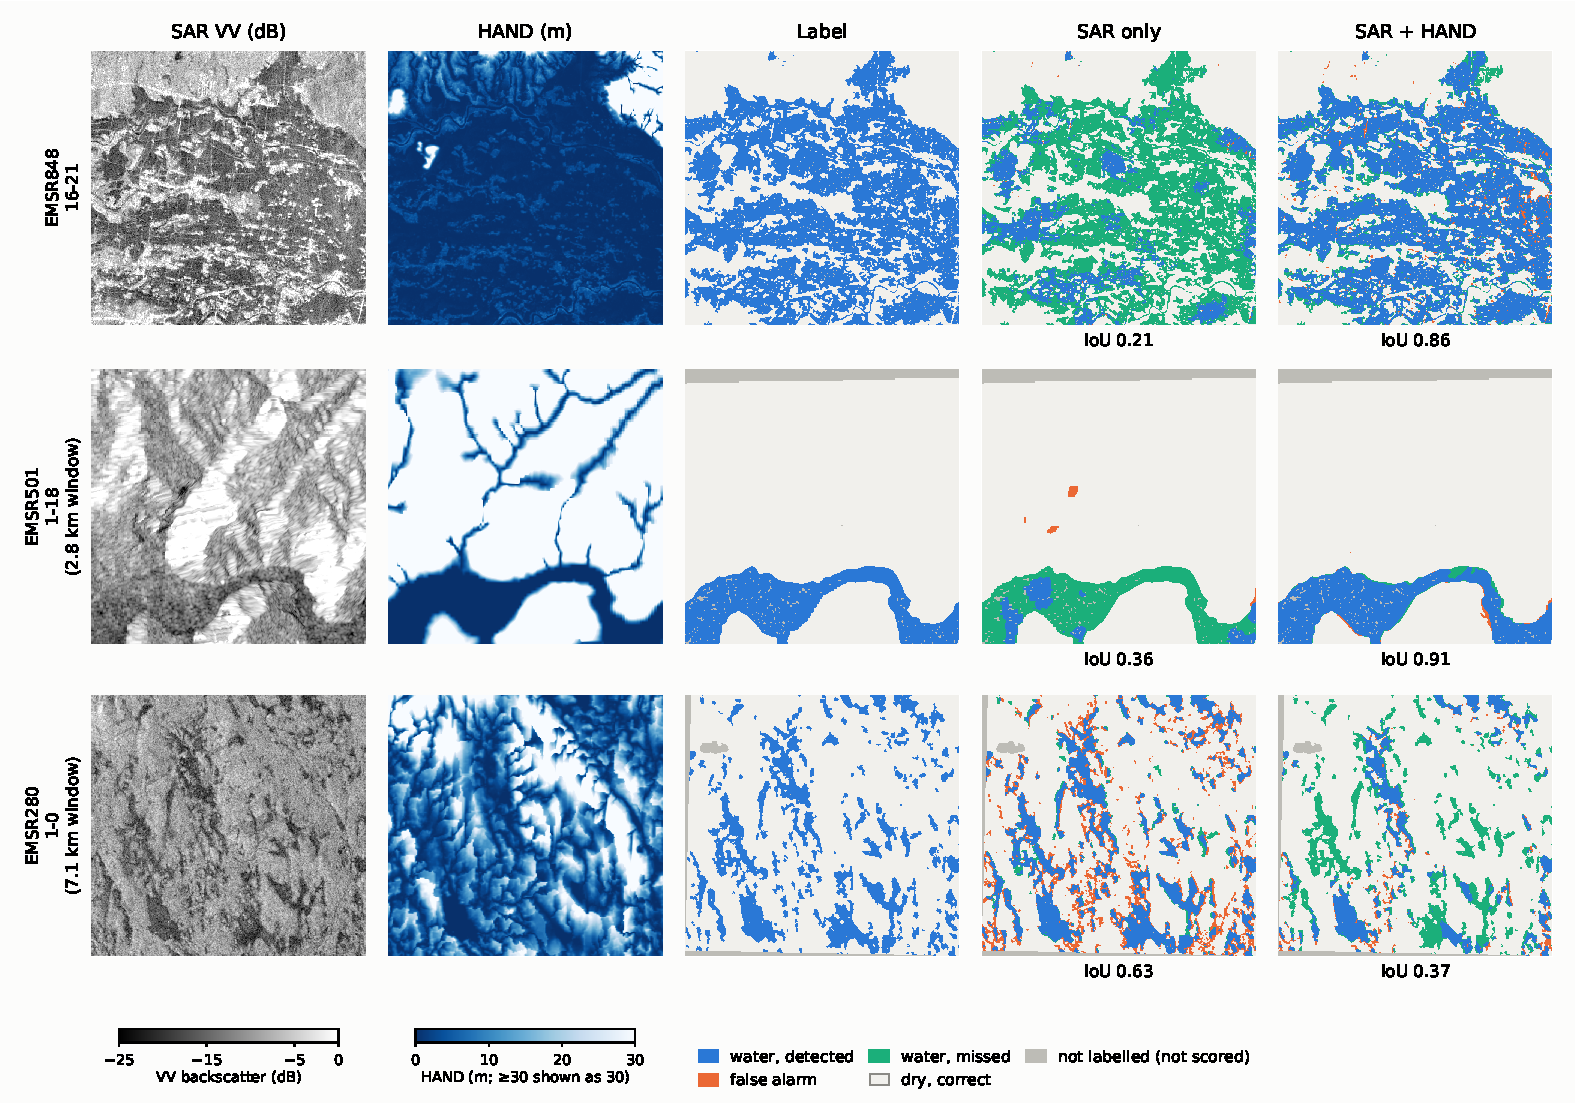
\includegraphics[width=\textwidth]{fig_example_tiles.pdf}
\caption{Example GEOID-Flood test tiles for the Sen1Floods11-trained U-Net (seed 0): SAR, HAND, label and
the errors of the SAR-only and SAR + HAND models. Top: floodplain gain; middle: mountain gain; bottom:
failure on Swedish lakes that sit above the DEM's drainage network (tile EMSR280\_1-0). Rows show windows of
different size (labelled; full 10.24-km tile in the top row), cropped to the labelled area; IoU is computed
over the whole tile.}
\label{fig:tiles}
\end{figure*}

\subsection{HAND, not just relief or known water}
\label{sec:ablation}

\begin{table}[t]
\caption{Which terrain helps in the Sen1Floods11 → GEOID-Flood transfer (pre-registered; trained on 11
events, 3 seeds; all 77/79 test events; two-way 95\% CIs).}
\label{tab:transfer_ablation}
\centering
\resizebox{\columnwidth}{!}{%
\begin{tabular}{@{}lccc@{}}
\toprule
Comparison & Flood, event-mean Δ & All water, event-mean Δ & Protocol pooled Δ \\
\midrule
DEM + slope vs SAR & +0.008 [−0.011, +0.026] & +0.014 [−0.027, +0.048] & +0.044 [+0.010, +0.086] \\
HAND vs DEM + slope & +0.024 [+0.005, +0.048] & +0.047 [+0.010, +0.099] & +0.028 [−0.004, +0.066] \\
HAND + DEM + slope vs HAND & −0.004 [−0.012, +0.004] & −0.004 [−0.014, +0.006] & +0.002 [−0.008, +0.014] \\
\bottomrule
\end{tabular}}
\end{table}

Is the transfer gain specific to HAND, or would any terrain input do? We fixed this test before training:
the same U-Net with DEM and slope instead of HAND, and with all three (Table~\ref{tab:transfer_ablation},
Fig.~\ref{fig:overview}b). DEM and slope recover only about a quarter of HAND's event-mean flood gain
(+0.008, CI including zero, against +0.032) and little of its all-water gain, and HAND beats them on both,
clearly for all water (+0.047 \ci{+0.010}{+0.099}, 68 of 79 events) and, for flood extent, with a CI close
to zero (+0.024 \ci{+0.005}{+0.048}, 55 of 77). Pooled over all pixels, which weights large events, DEM
and slope do better (+0.044 of HAND's +0.072 under the protocol): relief alone helps on the largest
floods, while HAND's drainage structure is what helps across events. Adding DEM and slope to HAND changes
nothing.

This differs from GEOID-Flood training (Table~S2). Trained on 20 GEOID-Flood events, DEM and slope recover
about two-thirds of HAND's flood gain (+0.021 vs.\ +0.032) and nine-tenths of its all-water gain, and HAND's
edge over them (+0.009 to +0.015 at 20 events) is not significant; at 159 events none of the terrain inputs changes flood
extent.

\emph{Not a permanent-water map.} A JRC Global Surface Water~\cite{pekel2016gsw} permanent-water channel
(occurrence ≥ 50\%, built identically for training and test; it reproduces Sen1Floods11's own JRC layer
at IoU 0.91) gives a third of HAND's all-water gain in the transfer (CIs over test events: +0.020 \ci{+0.010}{+0.030}, 61/79)
and slightly lowers flood IoU (−0.005 \ci{−0.009}{−0.001}); HAND beats it on both (+0.041
\ci{+0.024}{+0.060} all water, +0.038 \ci{+0.023}{+0.054} flood). With GEOID-Flood training (Table~S2),
JRC matches HAND's all-water gain at 20 events but explains none of the flood gain, and at 159 events it
\emph{hurts} flood extent (−0.054 \ci{−0.089}{−0.024} event-mean, −0.078 pooled): pooled flood recall on
unseen activations falls from 0.69 to 0.57 at unchanged precision (0.73 → 0.74). We read this as a shortcut:
the model learns that water is where the map says water already is and misses new flood water, which a
static water map invites and HAND, which marks where water \emph{could} collect, does not.

\subsection{The gain needs correctly located, detailed HAND}
\label{sec:mechanism}

\begin{table}[t]
\caption{HAND gain over SAR only when the HAND input is perturbed (pre-registered; Sen1Floods11-trained
U-Net, 3 seeds; all 77/79 GEOID-Flood test events; event-mean IoU, two-way 95\% CIs). Scored pixels are
identical in every row.}
\label{tab:mechanism}
\centering
\resizebox{\columnwidth}{!}{%
\begin{tabular}{@{}lcc@{}}
\toprule
HAND given to the model & Flood, Δ vs SAR only & All water, Δ vs SAR only \\
\midrule
Correct HAND & +0.032 [+0.018, +0.050] & +0.061 [+0.040, +0.086] \\
Shifted 100 m in x and y & +0.025 [+0.012, +0.041] & +0.031 [+0.012, +0.052] \\
Shifted 500 m in x and y & +0.003 [−0.011, +0.018] & −0.003 [−0.019, +0.013] \\
Blurred, $\sigma$ = 250 m & −0.001 [−0.015, +0.014] & −0.034 [−0.058, −0.010] \\
Another event's HAND (test only) & −0.061 [−0.081, −0.041] & −0.122 [−0.151, −0.095] \\
Another event's HAND (training and test) & −0.005 [−0.015, +0.006] & −0.001 [−0.021, +0.015] \\
\bottomrule
\end{tabular}}
\end{table}

Beating DEM and slope does not by itself show that the model uses what HAND says about the scene: the gain
could come from normalization, regularization or an easy-to-learn extra channel. We therefore fixed four
perturbations of the HAND input and one training control before running them (Table~\ref{tab:mechanism}).
Both hypotheses were supported. With HAND from a tile of another event the trained model becomes much worse
than SAR only (flood −0.061, all water −0.122), so it relies on HAND's content; shifted by 500\,m in both
axes (about 700\,m), the event-level gain disappears (+0.003 flood, −0.003 all water). A model trained and tested with another
event's HAND, which sees realistic HAND values that carry no information about the scene, gains nothing
(−0.005 \ci{−0.015}{+0.006} flood): the gain is not a side effect of having a terrain-like channel. A
100-m misregistration keeps most of the flood gain (+0.025) but halves the all-water gain, and blurring
away detail below about 250\,m removes the gain, so fine drainage structure matters. Pooled over all pixels,
the 500-m shift keeps about two-thirds of the flood gain (+0.050 \ci{+0.020}{+0.083} of +0.074; Table~S9), as large low-lying
areas stay low after a shift. Together with Table~\ref{tab:transfer_ablation}, this indicates that the gain comes
from correctly located, spatially detailed height above drainage across events, not from the extra
channel and not only from relief, which helps mainly on the largest low-lying floods.

\subsection{A foundation model does not replace terrain}
\label{sec:fm}

Does a large pretrained encoder make terrain redundant? We fine-tune TerraMind-1.0-base
\cite{jakubik2025terramind} (an 86\,M-parameter vision-transformer encoder pretrained on
TerraMesh~\cite{terramesh}, which includes Sentinel-1 GRD) with the U-Net decoder of the authors'
Sen1Floods11 configuration in TerraTorch~\cite{terratorch} (encoder layers 2, 5, 8 and 11; 101\,M
parameters in total, against 7.8\,M for our U-Net). VV and VH enter through the pretrained Sentinel-1 patch
embedding, standardized with TerraMind's own statistics; HAND enters as an extra band whose patch weights
start from random initialization, so the pretrained weights for VV and VH are unchanged. The learning
rate ($5\cdot10^{-5}$, from $2\cdot10^{-5}$, $5\cdot10^{-5}$ and $10^{-4}$) was chosen on the validation IoU
of the SAR-only model on one 20-event GEOID-Flood draw and reused unchanged for all TerraMind runs; all
other settings, data and step budgets equal the U-Net runs.

\begin{table}[t]
\caption{TerraMind ± HAND trained on the 11 Sen1Floods11 events (pre-registered; 3 seeds; all 77/79
GEOID-Flood test events; two-way 95\% CIs). TM: TerraMind-1.0-base, fine-tuned.}
\label{tab:fm_s1}
\centering
\resizebox{\columnwidth}{!}{%
\begin{tabular}{@{}lccc@{}}
\toprule
Comparison & Flood, event-mean Δ & All water, event-mean Δ & Protocol pooled Δ \\
\midrule
TM + HAND − TM & +0.031 [−0.000, +0.066] & +0.040 [+0.004, +0.081] & +0.026 [−0.009, +0.069] \\
TM − U-Net (SAR only) & −0.013 [−0.046, +0.018] & +0.009 [−0.030, +0.048] & +0.038 [−0.017, +0.094] \\
U-Net + HAND − TM & +0.045 [+0.022, +0.075] & +0.052 [+0.024, +0.087] & +0.034 [+0.005, +0.069] \\
\bottomrule
\end{tabular}}
\end{table}

In the main transfer setting (Table~\ref{tab:fm_s1}, Fig.~\ref{fig:overview}b), HAND helps TerraMind about
as much as it helps the U-Net in flood extent (+0.031 vs.\ +0.032 event-mean, the CI just reaching zero;
+0.036 \ci{+0.006}{+0.075} under the protocol, event-mean) and somewhat less for all water (+0.040 vs.\
+0.061). Without HAND, TerraMind is no better than the plain U-Net, and the 7.8\,M-parameter U-Net with HAND
beats it in all three measures of Table~\ref{tab:fm_s1} (flood +0.045 \ci{+0.022}{+0.075}, all water +0.052
\ci{+0.024}{+0.087}). With few training events, pretraining does not substitute for terrain in this configuration. These
comparisons use one fine-tuning setup (base model, U-Net decoder, one learning rate, HAND as an extra
patch-embedded band); more tuning or other fusion designs could change the ranking.

With GEOID-Flood training (Table~S3, Fig.~S3) the picture is similar: at 20 events HAND helps TerraMind
about as much as the U-Net in flood IoU (+0.031 vs.\ +0.032; both CIs only just exclude zero), less under
the protocol (+0.040 vs.\ +0.066), and not at 159 events. Our GEOID-trained TerraMind scores 0.491 under the
protocol on all 77 test events, slightly above GEOID-Flood's own TerraMind-B (0.478 frozen, 0.479
fine-tuned) and best single-image Sentinel-1 model (0.484).


\subsection{With 159 training events, HAND's flood-extent gain is not detectable}
\label{sec:geoid}

\begin{table*}[t]
\caption{Trained on GEOID-Flood train (159 events, 8,712 tiles, 3 seeds). Event-mean and pooled IoU,
SAR → SAR + HAND, with two-way 95\% CIs over seeds and test events.}
\label{tab:geoid}
\centering
\footnotesize
\begin{tabular}{@{}lccccc@{}}
\toprule
Test set & Events & Event-mean IoU & Δ (95\% CI) & Pooled IoU & Δ (95\% CI) \\
\midrule
GEOID test, unseen activations, all water & 39 & 0.625 → 0.648 & +0.023 [+0.004, +0.045] & 0.713 → 0.763 & +0.050 [+0.003, +0.118] \\
GEOID test, unseen activations, flooded only & 38 & 0.381 → 0.380 & −0.001 [−0.019, +0.016] & 0.549 → 0.559 & +0.011 [−0.017, +0.037] \\
GEOID test, shared activations, flooded only & 39 & 0.321 → 0.326 & +0.005 [−0.008, +0.024] & 0.468 → 0.438 & −0.030 [−0.059, −0.002] \\
GEOID held-out 2026, flooded only & 9 & 0.488 → 0.481 & −0.008 [−0.022, +0.007] & 0.644 → 0.626 & −0.017 [−0.034, +0.014] \\
Sen1Floods11 minus overlapping events & 8 & 0.512 → 0.530 & +0.018 [+0.008, +0.030]$^\dagger$ & 0.571 → 0.590 & \\
\bottomrule
\end{tabular}
\\[2pt]\raggedright\footnotesize $^\dagger$CI resamples test events only.
\end{table*}

Trained on GEOID-Flood's 159 training events, the picture changes (Table~\ref{tab:geoid}). This endpoint
differs from the 11-event one in training data (GEOID-Flood rather than Sen1Floods11) and in test events
(the 38/39 unseen activations rather than all 77/79), not only in the number of events; the learning curve
below varies the event count within GEOID-Flood. On flood
extent, HAND does nothing on unseen activations on either metric (event-mean −0.001, pooled +0.011, both
CIs include zero); threshold-free, flood AP is unchanged too (event-mean −0.000 \ci{−0.014}{+0.012}, CI over test events). On
all water it still helps, though with CIs close to zero (+0.023 \ci{+0.004}{+0.045} event-mean, +0.050
\ci{+0.003}{+0.118} pooled). On test activations that share AoIs with training, HAND \emph{lowers} pooled
flood IoU (0.468 → 0.438) while event-mean IoU is unchanged; one event, EMSR419, dominates
(Section~\ref{sec:failures}).

Under the GEOID-Flood protocol our GEOID-trained U-Net scores \iouf{} 0.452 ± 0.005 (SAR) and 0.469 ±
0.008 (+ HAND) on the 77 test events with flood, inside the 0.41--0.48 that GEOID-Flood reports for
single-image Sentinel-1 models with ImageNet or foundation-model encoders (one frozen encoder, Satlas,
scores 0.21), so our pipeline and baselines are comparable. HAND's protocol gain at 159 events is small,
with a CI just above zero on all 77 events (+0.017 \ci{+0.001}{+0.035}) and including zero on unseen
activations alone (+0.021 \ci{−0.001}{+0.043}). Scoring the post-event map alone against flood labels,
with permanent water as a false positive, instead gives −0.009 \ci{−0.021}{−0.000} on all 77 events
(−0.008 \ci{−0.024}{+0.007} on unseen activations): the protocol gain comes from better water detection in
both images, which the pre-image subtraction turns into flood IoU, not from better flood delineation. On
the nine held-out 2026 events the protocol gain is −0.017 \ci{−0.039}{+0.018}.

\begin{figure}[t]
\centering
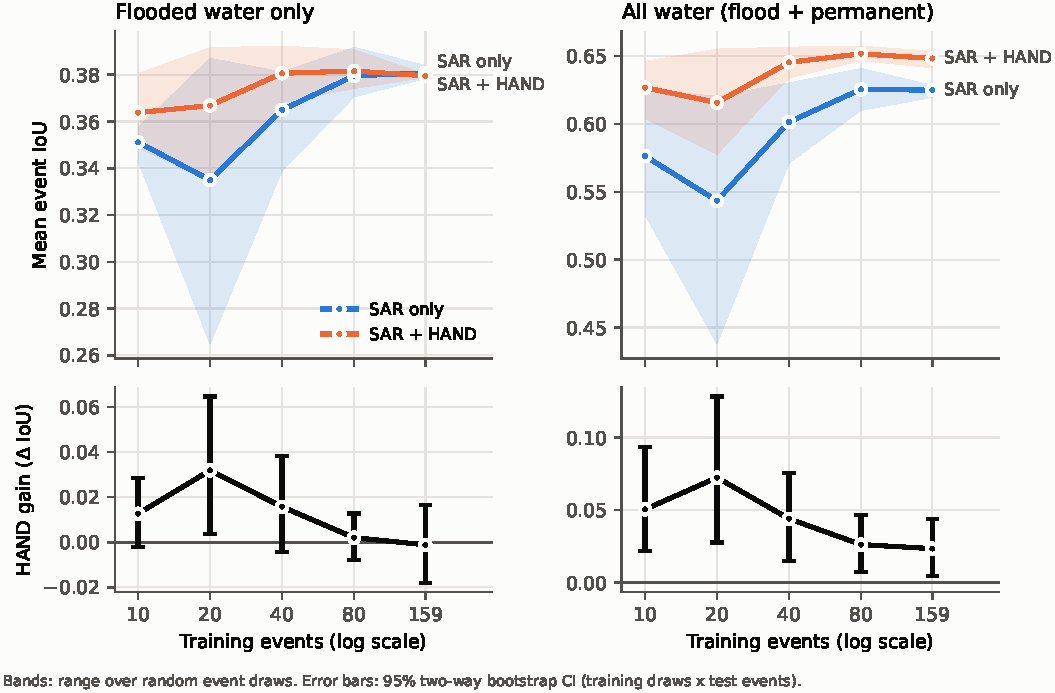
\includegraphics[width=\columnwidth]{fig_learning_curve.pdf}
\caption{IoU and HAND gain against the number of GEOID-Flood training events (unseen test activations,
event-mean IoU). Top: mean over draws, band = range over draws. Bottom: HAND gain with two-way 95\% CIs
over draws and test events.}
\label{fig:curve}
\end{figure}

\begin{table}[t]
\caption{HAND gain against the number of GEOID-Flood training events, flooded water only, 38 unseen test
activations (5 draws; 159 events: 3 seeds). Two-way 95\% CIs.}
\label{tab:curve}
\centering
\resizebox{\columnwidth}{!}{%
\begin{tabular}{@{}lccc@{}}
\toprule
Training events (tiles) & Event-mean Δ & Pooled IoU, SAR → + HAND & Pooled Δ \\
\midrule
10 (262–728) & +0.013 [−0.002, +0.028] & 0.490 → 0.529 & +0.039 [+0.008, +0.070] \\
20 (651–1,759) & +0.032 [+0.004, +0.065] & 0.468 → 0.530 & +0.062 [+0.019, +0.111] \\
40 (1,834–3,168) & +0.016 [−0.004, +0.038] & 0.513 → 0.561 & +0.048 [+0.015, +0.083] \\
80 (3,387–4,827) & +0.002 [−0.008, +0.012] & 0.539 → 0.561 & +0.022 [−0.002, +0.052] \\
159 (8,712) & −0.001 [−0.019, +0.016] & 0.549 → 0.559 & +0.011 [−0.017, +0.037] \\
\bottomrule
\end{tabular}}
\end{table}

\emph{Learning curve.} To see how the value of HAND depends on the number of training events, we train on
random subsets of 10, 20, 40 and 80 GEOID-Flood training events (5 draws each; draw $k$ trained with seed
$k$) and on the full 159, all with the same step budget (Fig.~\ref{fig:curve}, Table~\ref{tab:curve}).
Exploratory, the flood-extent HAND gain looked largest at 20--40 events and gone by 159: at 20 events its
CI only just excludes zero (+0.032 \ci{+0.004}{+0.065}), at 40 the pooled CI excludes zero but the
event-mean one does not, and at 80 both include zero. Which events are in a small training set matters:
at 20 events the per-draw flood gain ranges from −0.008 to +0.069. With HAND, 20 events approach the pooled
flood IoU that SAR-only reaches with 80--159 (0.530 vs.\ 0.539--0.549).

\emph{The pre-registered confirmation failed.} To test the decline, we fixed a contrast before training
new models: on three new, independent equal-tiles draws (500 tiles) at each of 20, 40 and 159 events, the
mean HAND gain at 20 and 40 events minus the gain at 159, on the 38 unseen test events, with a one-sided
Wilcoxon test over events. The contrast was +0.0025 \ci{−0.007}{+0.013} (CI over test
events), $p = 0.37$ (all water $p = 0.37$), against +0.012 \ci{+0.004}{+0.019}, $p = 0.003$, on the
exploratory draws that motivated it; a post hoc average-precision version is also null ($p = 0.49$; details
with Table~S4). We therefore do not claim that the HAND gain declines steadily with event count; the robust
statements are the endpoints---a clear gain when training on 11 Sen1Floods11 events and testing
externally, and no detectable flood-extent gain with 159 GEOID-Flood events.

\emph{Events, not tiles.} A control cuts every subset to exactly 500 tiles spread evenly over its events
(3 draws; Table~S4, Fig.~S1). 500 tiles from all 159 events match all 8,712 for the SAR-only model (flood
event-mean 0.381 vs.\ 0.381; all water 0.632 vs.\ 0.625). Because the step budget is fixed and each subset
has different events, this shows that extra tiles from the same events add nothing at this budget; it does
not isolate event diversity as a cause. Regressing event-mean IoU on log events and log
tiles over all 38 exploratory draws (Table~S5), the SAR-only model improves with each doubling of events
(flood +0.007 \ci{+0.001}{+0.015}, all water +0.014 \ci{+0.004}{+0.028}; suggestive by our criterion) and
not with more tiles (−0.001 and −0.004, CIs including zero).

\subsection{The pre-event image partly substitutes for terrain}
\label{sec:cd}

GEOID-Flood provides a pre-event Sentinel-1 image for every tile, so a model can be given both images at
once. Operationally, Sentinel-1's routine acquisitions usually supply a recent pre-event image of the same
orbit, but seasonal changes in vegetation and soil moisture between the two dates add their own errors. We train the same U-Net on [VV, VH, VV\textsubscript{pre}, VH\textsubscript{pre}] (± HAND) to predict
flooded water directly, with permanent water and background as negatives, i.e., GEOID-Flood's flood class.
All 8,712 training tiles have a pre-event image; requiring both images removes 0.8\% of valid pixels. It
is scored on exactly the tiles and pixels of the protocol-matched single-image numbers, so the rows of
Table~\ref{tab:cd} are directly comparable.

\begin{table}[t]
\caption{HAND gain with and without the pre-event image (unseen activations; pooled \iouf{} under the
GEOID-Flood protocol, mean over draws/seeds; Δ from confusion counts averaged over draws/seeds, two-way
95\% CI; last column event-mean Δ).}
\label{tab:cd}
\centering
\footnotesize
\setlength{\tabcolsep}{2.5pt}
\resizebox{\columnwidth}{!}{%
\begin{tabular}{@{}lccccc@{}}
\toprule
Model & Events & SAR & + HAND & Δ pooled (95\% CI) & Δ ev. \\
\midrule
Single image, differenced & 20 & 0.382 & 0.448 & +0.066 [+0.019, +0.111] & +0.036 \\
Change detection & 20 & 0.404 & 0.426 & +0.024 [−0.037, +0.085] & +0.000 \\
Single image, differenced & 159 & 0.475 & 0.496 & +0.021 [−0.001, +0.043] & +0.013 \\
Change detection & 159 & 0.463 & 0.491 & +0.029 [−0.011, +0.057] & +0.005 \\
\bottomrule
\end{tabular}}
\end{table}

A trained change model is no better than differencing two single-image maps (without HAND: −0.014
\ci{−0.069}{+0.037} at 159 events, +0.020 \ci{−0.048}{+0.098} at 20), but it is much less sensitive to
which 20 events it is trained on (standard deviation over draws 0.041 vs.\ 0.090). With the pre-event
image, HAND matters less at 20 events (+0.024 vs.\ +0.066, no longer significant) and about as much at 159
(+0.029 vs.\ +0.021); the event-mean gains are near zero. Plausibly the pre-event image supplies part of what
HAND supplies with few training events: which dark, smooth surfaces were already there before the flood.

\subsection{Failure cases resist two pre-registered remedies}
\label{sec:failures}

HAND fails in two ways. On flat ground where every pixel is near drainage it pushes the model toward flood
everywhere: Somalia in LOEO, and EMSR419 (Iran, January 2020) with GEOID-Flood training, whose tiles have a
median HAND of 0.44\,m with 81\% of pixels below 2\,m (5.8\,m and 38\% over the test set) and which
contributes 1.37\,M of the 1.56\,M extra false-positive pixels on shared activations (event IoU 0.188 →
0.142). And it suppresses water bodies the DEM drainage network misses: on a Swedish tile
(EMSR280\_1-0; Fig.~\ref{fig:tiles}, bottom) HAND suppresses lakes that sit above the network (tile IoU
0.61 → 0.30 over 3 seeds), although over the whole Swedish event (113 tiles) HAND still helps (0.548 →
0.663).

\emph{Relief gate.} The obvious remedy for the first failure is to ignore HAND on flat ground. We fixed the
rule before computing any outcome: a tile is \emph{flat} when the 90th percentile of its valid HAND is below
2\,m, and flat tiles take the SAR-only model's prediction from the same seed or draw (5\% of test tiles, in
28 of 80 events; no retraining or tuning). The primary outcome, pooled \iouf{} under the protocol on
unseen activations, does not improve (gated minus ungated: −0.016 \ci{−0.047}{+0.001} at 20 events, −0.003
\ci{−0.007}{+0.001} at 159; Table~S6), and on all 77 test events at 20 training events the gate lowers it
(−0.012 \ci{−0.030}{−0.001}). Gating more tiles costs more (exploratory: threshold 5\,m −0.022
\ci{−0.053}{−0.002}): HAND helps on flat tiles on average, and the failure is concentrated in a few events,
not a property of flat tiles.

\emph{HAND dropout.} For the second failure, which puts real water at high HAND, a standard remedy is
modality dropout~\cite{neverova2016moddrop}: during training the HAND channel of a random 50\% of tiles is
replaced by −1 (outside the normalized range), and HAND is always present at test time. Fixed before
training (Table~S7), it does not help: dropout raises no mean gain by more than +0.001, and with 11 training
events it removes a quarter to two-fifths of HAND's gain over SAR only (flood event-mean −0.008
\ci{−0.016}{−0.001}, all water −0.020 \ci{−0.036}{−0.009}). At 159 events it shrinks the model toward SAR
only: fewer large losses (protocol tail 5 → 2 events) but also fewer gains (events improved 25 → 21). The
Swedish tile recovers partly (0.30 → 0.46), but the Swedish event as a whole gets worse in every setting,
because HAND helps most of that event's tiles.

\section{Discussion}
\label{sec:discussion}

\subsection{What same-event evaluation misses}
On Sen1Floods11's own split HAND looks useless (+0.007); on an event outside training (Bolivia) and on 79
external floods it helps clearly. The contrast is what a practitioner would see when choosing inputs from
the standard benchmark. It does not fully isolate the effect of the split: the external events also differ
from Sen1Floods11 in region, scenes and labelling, so dataset shift and the change from known to new events
act together. Bolivia, which holds the dataset fixed, points the same way but is a single event; a
controlled within-dataset comparison of same-event and held-out-event splits at matched budgets would
separate the two.

\subsection{What makes HAND useful}
The model uses what HAND says about the place. The event-level gain disappears when HAND is shifted by
500\,m in each axis, blurred or taken from another flood, and a model trained on mismatched HAND gains
nothing; DEM and slope recover only a quarter of it. HAND is height relative to the local drainage
network, which relief and slope only approximate, and its position to within a few hundred metres and its
detail at that scale matter. Where it helps is consistent with this: HAND removes false alarms on higher
ground and on steep, shadowed slopes. Pooled over pixels, part of the gain survives a 500-m shift and DEM
and slope recover more of it, plausibly because the largest floods cover broad low-lying plains that stay low after
a shift and that relief alone identifies; the event-level gain, which weights every flood equally, depends
on the finer drainage structure. Terrain priors say where water \emph{can} be; a permanent-water map says
where it \emph{has been}, and with 159 training events it appears to teach the model to look for water only there
(pooled flood recall 0.69 → 0.57 at unchanged precision). As a physics loss, by contrast, HAND adds nothing: trained models already
satisfy the tested constraints (monotonicity is violated on fewer than 0.5\% of pixel pairs), and enforcing
them removes violations that are not where the errors are. Here the prior helps as an input, which
carries information the SAR does not.

\subsection{When the advantage shrinks or fails}
\emph{Many training events.} A model that has seen few floods may not have learned which backscatter
patterns are terrain artefacts, and HAND tells it directly; a model that has seen many floods could learn
this from SAR alone. The endpoints fit this hypothesis---a clear gain with 11 Sen1Floods11 events, none
detectable on flood extent with 159 GEOID-Flood events---but they differ in dataset too, and the
pre-registered test of a decline in between was null; draw-to-draw variance at 20--40 events is large. With
20 GEOID-Flood training events, DEM and slope also recover most of HAND's gain, which suggests that more
varied training lets a model infer where water collects from relief; we did not test this directly.
\emph{The pre-event image} partly substitutes for terrain with few events (pooled gain at 20 events +0.024, not significant, vs.\ +0.066).

\emph{Failure cases.} HAND fails on flat terrain where everything is near drainage (Somalia, EMSR419), on
water bodies the DEM drainage network misses (the Swedish lakes), and in mangroves (pooled over the seven
events that contain them). Neither pre-registered remedy works: gating HAND on flat tiles removes gains, and HAND dropout
shrinks the model toward SAR only. The losses sit in a few events that terrain statistics do not pick out
in advance; a fix would need to know when the DEM's drainage network is wrong. The stratified results are
descriptive: land-cover classes are tied to geography and flood type, so they show where the gain occurs,
not why, and the absolute IoU in built-up areas stays low even with HAND.

\emph{Registration.} Because the gain depends on HAND's position, terrain and radar must be co-registered.
Sentinel-1 IW GRD products are specified to about 7\,m absolute location accuracy~\cite{s1iwgrd}, and HAND
cells are 30\,m; both are far below the 500-m shift that removes the event-level gain, and a 100-m shift
costs little. Resampling HAND onto each SAR tile's own grid, as here, avoids larger errors.

\subsection{Limitations}
Besides the caveats stated with each result (one TerraMind configuration; a fixed step budget; 3--5 seeds),
GEOID-Flood labels are CEMS rapid-mapping products~\cite{cems}, not hand labels; their quality varies by
activation, and we did not audit them, so some apparent false alarms may be unmapped water. 50 of the 79
test events are in Europe. The change-detection baseline stacks the pre-event image as two extra channels.
HAND inherits the drainage-network errors of the GLO-30 DEM, and we did not compare it with other
hydrologically derived terrain features such as distance to drainage, or with HAND from other DEMs.

\section{Conclusion}
\label{sec:conclusion}

Evaluated on floods the model has never seen, terrain helps a SAR flood-segmentation network as an input:
a U-Net trained on the 11 Sen1Floods11 events improves water and flood mapping on 79 external CEMS
activations. Its event-level part needs correctly located, detailed height above drainage, which relief, a
permanent-water map or, with few training events, a larger pretrained model does not replace.
As a post-processing mask HAND recovers part of the gain, as a physics loss little, and with 159 training
events its flood-extent gain is not detectable. Whether same-event splits understate the gain, as the
Bolivia hold-out suggests, would need more than Sen1Floods11's ten test events to settle. With few labelled
floods, terrain is a cheap gain, and it should be judged on held-out floods.

\section*{Data and Code Availability}
All data are public: Sen1Floods11~\cite{bonafilia2020sen1floods11}, GEOID-Flood~\cite{geoidflood} (CC BY
4.0), Copernicus GLO-30~\cite{glo30dem}, ASF GLO-30 HAND~\cite{asfhand}, ESA WorldCover~\cite{zanaga2022worldcover}
and JRC Global Surface Water~\cite{pekel2016gsw}. Code (MIT license), every SLURM submission and the scripts
that regenerate every table are at \url{https://github.com/jeremyky/SAR-Flood-Terrain}; run outputs and
checkpoints are available from the authors and will be archived with a DOI on publication.

\section*{Acknowledgment}
The authors acknowledge Research Computing at the University of Virginia for providing computational
resources and technical support that have contributed to the results reported in this publication.


\bibliographystyle{IEEEtran}
\bibliography{refs}

\end{document}
